\chapter{Feasibility}
\label{ch:feasibility}

This chapter shows that the plan in Chapter~\ref{ch:method} is achievable, through the planned environment, the datasets, the system design and the prototypes built so far.

\section{Coding Environment}
\label{sec:env}

The system will be developed in Python. OpenCV \cite{bradski_opencv_2000} will be used for image processing, PyTorch for the networks and Grad-CAM, and matplotlib for the interface; these were chosen for their mature libraries and their support for displaying ECG images and plots. Training will run on my own PC, which has a GPU, and the code will be kept under version control on GitHub (Appendix~\ref{app:repo}).

\section{Datasets}
\label{sec:datasets}

\begin{table}[H]
  \centering
  \footnotesize
  \begin{minipage}[t]{0.40\linewidth}
    \vspace{0pt}
    \centering
    \caption{Records per class in PTB-XL.}
    \label{tab:class-counts}
    \begin{tabular}{@{}lr@{}}
      \toprule
      \textbf{Class} & \textbf{Records} \\
      \midrule
      Normal & 9514 \\
      Myocardial infarction & 5469 \\
      ST/T change & 5235 \\
      Conduction disturbance & 4898 \\
      Hypertrophy & 2649 \\
      Atrial fibrillation & 1514 \\
      Atrial flutter & 73 \\
      Sinus tachycardia & 826 \\
      Sinus bradycardia & 637 \\
      \bottomrule
    \end{tabular}
  \end{minipage}\hfill
  \begin{minipage}[t]{0.55\linewidth}
    \vspace{0pt}
    \normalsize
    PTB-XL provides 21,800 labelled twelve-lead ECGs with patient-wise folds \cite{wagner_ptbxl_2020}; Table~\ref{tab:class-counts} gives the records per class. The ECG-Image-Database provides 35,595 real images of 1,977 recordings, 977 from PTB-XL and 1,000 from Emory Healthcare \cite{reyna_ecg-image-database_2024}. The PTB-XL part can be matched to PTB-XL labels by record, giving the labelled real test set; real images per class, and whether the Emory labels map to the nine classes, will be checked in Phase 1. Because the real images are of PTB-XL recordings, their patients will be removed from the training folds, so that no ECG is seen in both training and testing. Rare classes may only be evaluated on rendered images.
  \end{minipage}
\end{table}

\section{Design}
\label{sec:design}

Figure~\ref{fig:architecture} shows the architecture, with each module's inputs and outputs. The modules will be separate, so any one can be replaced without changing the others (NFR10). The GUI will offer a user view, with explanations, and a clinical view, with every class score, its threshold and fuller measured values. Offline training will produce the model weights, temperature $T$ and class thresholds that the application loads.

\begin{figure}[H]
  \centering
  \makebox[\linewidth][c]{%
  \begin{tikzpicture}[
      font=\small,
      mod/.style={draw, rounded corners=2pt, align=center, text width=28mm,
                  minimum height=10mm, fill=#1},
      mod/.default=blue!10,
      arr/.style={-{Latex[length=2mm]}, thick},
      lab/.style={font=\scriptsize, fill=white, inner sep=1pt}
    ]
    % analysis pipeline (middle column)
    \node[mod] (pre) at (0,0)      {Preprocessing\\\footnotesize OpenCV};
    \node[mod] (det) at (0,-14.5mm)  {Detection\\\footnotesize R peaks, HR, RR};
    \node[mod=orange!12] (clf) at (0,-29mm) {Classifier\\\footnotesize CNN (PyTorch)};
    \node[mod=orange!12] (cal) at (0,-43.5mm) {Calibration\\\footnotesize temperature $T$};
    \node[mod=orange!12] (exp) at (0,-58mm) {Explanation\\\footnotesize Grad-CAM};
    \node[draw, dashed, rounded corners, inner sep=3mm, fit=(pre)(exp),
          label={[font=\footnotesize\itshape]above:Analysis pipeline}] (pipe) {};

    % GUI (left)
    \node[mod=green!12, minimum height=69mm, text width=26mm, anchor=north]
         (gui) at (-56mm,5.5mm) {};
    \node[align=center, font=\small, text width=24mm, anchor=north] at (gui.north)
         {\textbf{GUI module}\\[3pt]Upload\\Results screen\\User view\\Clinical view};

    % offline training (right)
    \node[mod=black!5] (data) at (56mm,-8mm) {Data preparation\\\footnotesize ECG-Image-Kit, PTB-XL, ECG-Image-Database};
    \node[mod=black!5] (train) at (56mm,-27mm) {Training};
    \node[mod=black!5] (store) at (56mm,-47mm) {Saved model\\\footnotesize weights, $T$, thresholds};
    \node[draw, dashed, rounded corners, inner sep=3mm, fit=(data)(store),
          label={[font=\footnotesize\itshape]above:Offline training}] {};

    % pipeline flow
    \draw[arr] (pre) -- node[lab, right]{cleaned image, scale} (det);
    \draw[arr] (det) -- node[lab, right]{timing features} (clf);
    \draw[arr] (clf) -- node[lab, right]{class scores} (cal);
    \draw[arr] (cal) -- node[lab, right]{flagged classes} (exp);

    % GUI <-> pipeline
    \draw[arr] (gui.east |- 0,2.5mm) -- node[lab, above]{image} ([yshift=2.5mm]pre.west);
    \draw[arr] ([yshift=-2.5mm]pre.west) -- node[lab, below]{quality warning} (gui.east |- 0,-2.5mm);
    \draw[arr] (det.west) -- node[lab, above]{HR, RR} (gui.east |- det);
    \draw[arr] (cal.west) -- node[lab, above]{flags, confidence} (gui.east |- cal);
    \draw[arr] (exp.west) -- node[lab, above]{heatmaps} (gui.east |- exp);

    % offline flow
    \draw[arr] (data) -- node[lab, right]{images, labels} (train);
    \draw[arr] (train) -- (store);
    \draw[arr, dashed] (store.north west) -- node[font=\scriptsize, above, sloped, pos=0.5]{weights} (clf.east);
    \draw[arr, dashed] (store.south west) -- node[font=\scriptsize, below, sloped, pos=0.5]{$T$, thresholds} (cal.east);
  \end{tikzpicture}%
  }
  \caption{Planned system architecture, showing the modules, their inputs and outputs, and how they connect.}
  \label{fig:architecture}
\end{figure}

\section{Prototypes}
\label{sec:prototypes}

Three prototypes test the main risks of the plan. Table~\ref{tab:prototypes} gives the status of each one and what it demonstrates, Figures~\ref{fig:rendered} and~\ref{fig:proto2} show the first two, and the wireframes are in Appendix~\ref{app:wireframes}.

\begin{table}[H]
  \centering
  \footnotesize
  \setlength{\arrayrulewidth}{0.8pt}
  \renewcommand{\arraystretch}{1.15}
  \caption{Status of the prototypes.}
  \label{tab:prototypes}
  \begin{tabular}{|p{0.22\linewidth}|p{0.12\linewidth}|p{0.56\linewidth}|}
    \hline
    \rowcolor{cyan!90!black}
    \textcolor{white}{\textbf{Prototype}} & \textcolor{white}{\textbf{Status}} &
    \textcolor{white}{\textbf{Demonstrates}} \\
    \hline
    1: Data and rendering & Completed & PTB-XL labels were mapped to the nine classes, and records were rendered with ECG-Image-Kit. The rendered beats match the source signal's timing, but the trace is cleaner than real images, which supports measuring the rendered-to-real gap. \\
    \hline
    2: Preprocessing & Completed & OpenCV thresholding removed colour and separated the trace, and feature detection removed the grid, leaving the trace alone. Beat detection is planned for Phase 2. \\
    \hline
    3: GUI wireframes & Completed & Show the user and clinical views, and how flags, confidence, heatmaps and measured values are presented, before the interface is built (Appendix~\ref{app:wireframes}). \\
    \hline
  \end{tabular}
\end{table}

\begin{figure}[H]
  \centering
  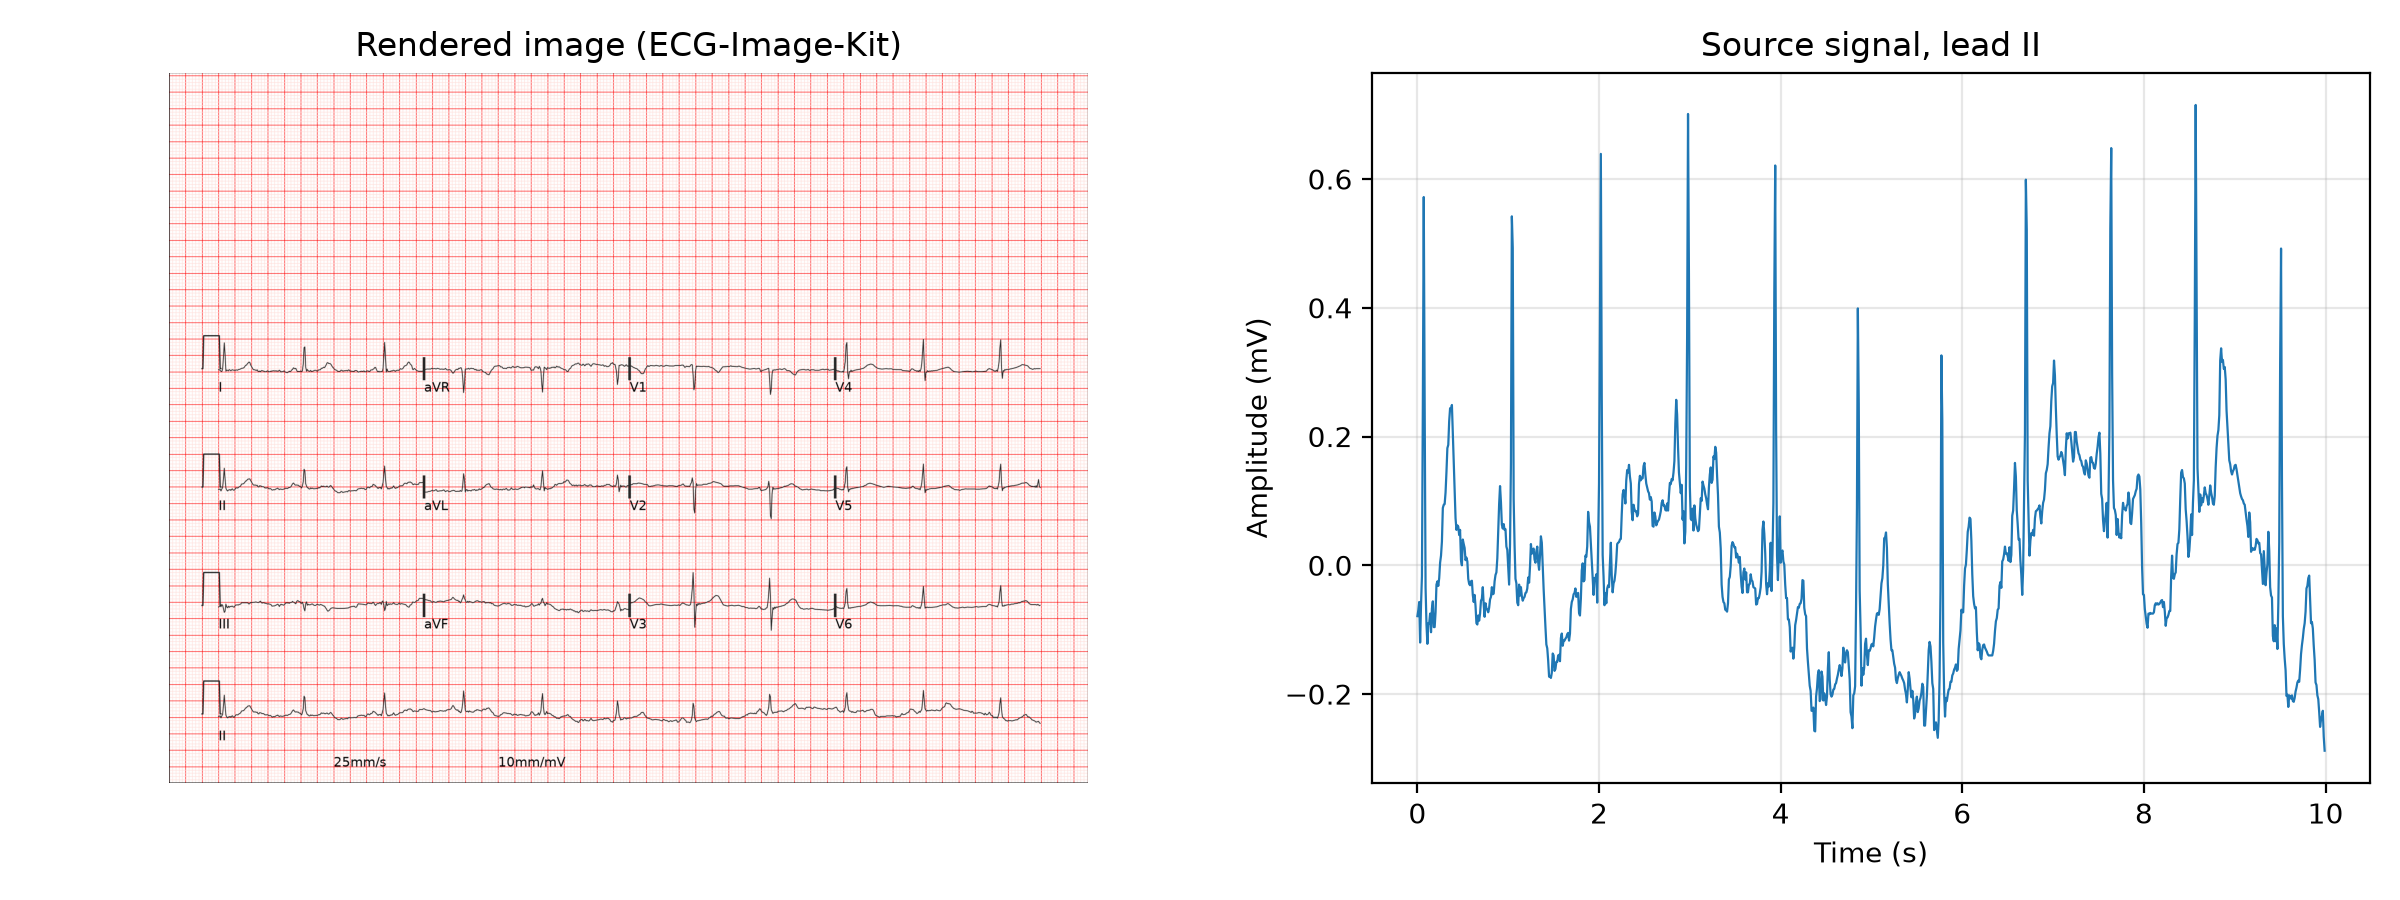
\includegraphics[width=0.85\linewidth,height=0.22\textheight,keepaspectratio]{images/rendered_vs_signal.png}
  \caption{Prototype 1: PTB-XL record 00001\_lr rendered with ECG-Image-Kit
    \cite{shivashankara_ecg-image-kit_2024} (left), and the lead II signal it was generated
    from (right). Both show 11 beats at about 0.9--1.0\,s spacing.}
  \label{fig:rendered}
\end{figure}

\begin{figure}[H]
  \centering
  \begin{subfigure}[b]{0.35\linewidth}
    \centering
    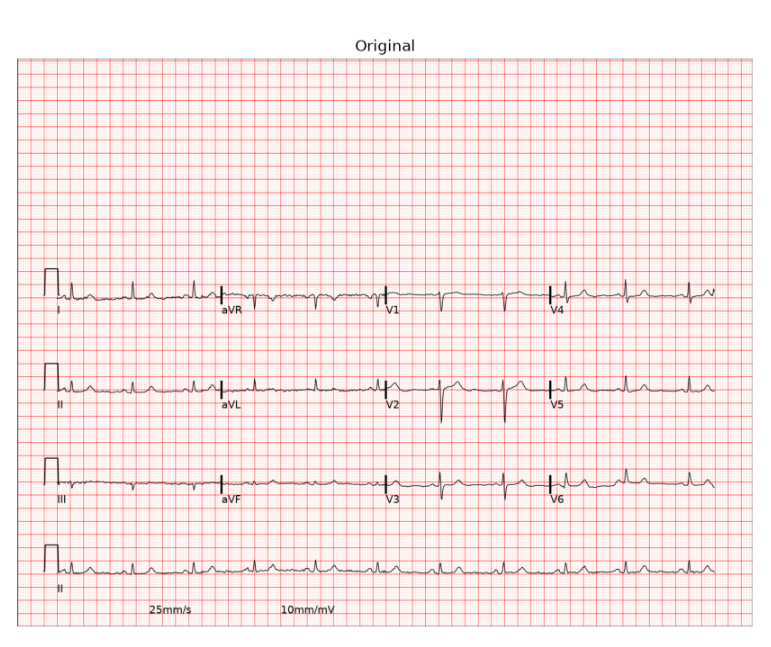
\includegraphics[width=\linewidth]{images/p2_initial.png}
    \caption{Initial Image.}
    \label{fig:img1}
  \end{subfigure}\hfill
  \begin{subfigure}[b]{0.35\linewidth}
    \centering
    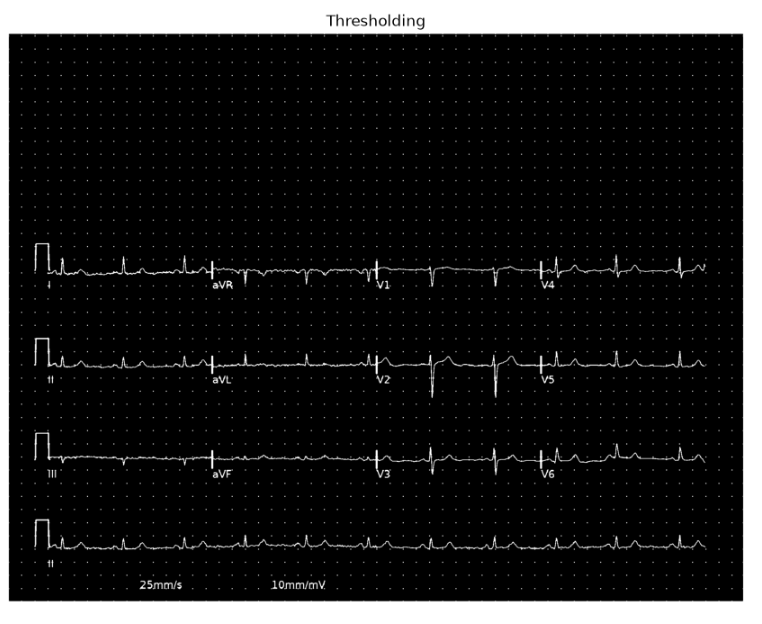
\includegraphics[width=\linewidth]{images/p2_thre.png}
    \caption{Image thresholded.}
    \label{fig:img2}
  \end{subfigure}\hfill
  \begin{subfigure}[b]{0.35\linewidth}
    \centering
    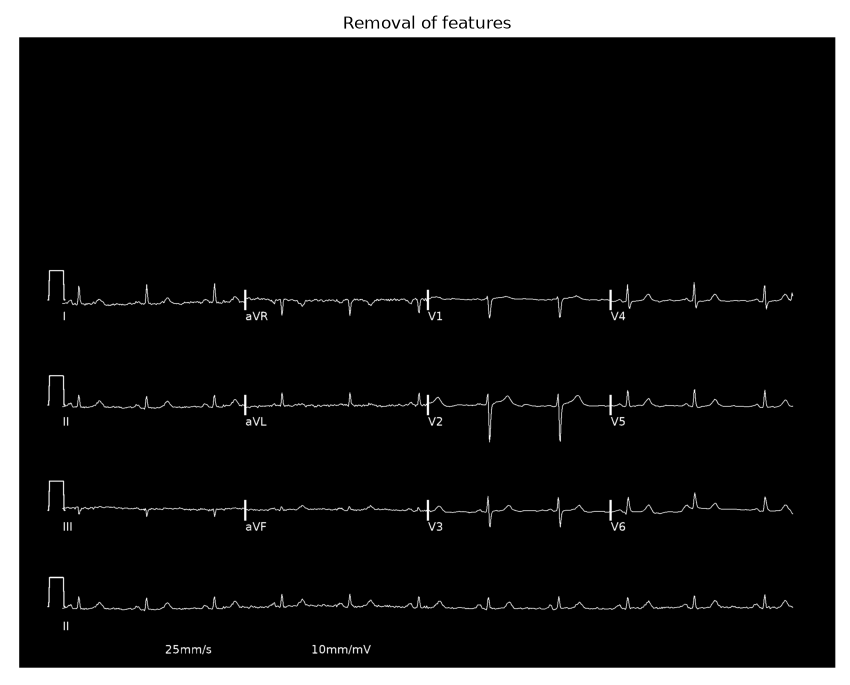
\includegraphics[width=\linewidth]{images/p2_remov.png}
    \caption{Features Removed.}
    \label{fig:img3}
  \end{subfigure}
  \caption{Extracting a waveform from an ECG.}
  \label{fig:proto2}
\end{figure}
\section{Risks}
\label{sec:feas-risks}

The full risk assessment is in Table~\ref{tab:risks} (Appendix~\ref{app:risks}). The main risks for feasibility are that models may not transfer from rendered to real images (R1), that detection may fail on poor images (R2), that rare classes have too few cases (R3), and that time may run short for the full interface (R10). Their fallbacks are reporting the gap as a result, classifying from the image alone, reporting rare classes with counts, and a reduced interface.